        %%******************************************%%
        %%                                          %%
        %%        Modello di tesi di laurea         %%
        %%            di Andrea Giraldin            %%
        %%                                          %%
        %%             2 novembre 2012              %%
        %%                                          %%
        %%******************************************%%

\begin{document}
    \frontmatter
    \begin{titlepage}
    \begin{center}
        \begin{LARGE}
            \textbf{\myUni}\\
        \end{LARGE}

        \vspace{10pt}

        \begin{Large}
            \textsc{\myDepartment}\\
        \end{Large}

        \vspace{10pt}

        \begin{large}
            \textsc{\myFaculty}\\
        \end{large}

        \vspace{30pt}
        \begin{figure}[htbp]
            \centering
            
\includegraphics[height=6cm]{unipd-logo}
        \end{figure}
        \vspace{30pt}

        \begin{LARGE}
            \textbf{\myTitle}\\
        \end{LARGE}

        \vspace{10pt}

        \begin{large}
            \textsl{\myDegree}\\
        \end{large}

        \vspace{40pt}

        \begin{large}
            \begin{flushleft}
                \textit{Relatore}\\
                \vspace{5pt}
                \profTitle\ \myProf
            \end{flushleft}

            % You can tweak the spacing to have professor and student names on the same line
            % useful if the page is broken by a long thesis title and you need more space
            % \vspace{-52pt}

            \begin{flushright}
                \textit{Laureando}\\
                \vspace{5pt}
                \myName
            \end{flushright}
        \end{large}

        \vspace{40pt}

        \line(1, 0){338} \\
        \begin{normalsize}
            \textsc{Anno Accademico \myAA}
        \end{normalsize}
    \end{center}
\end{titlepage}

    \clearpage
\phantomsection
\thispagestyle{empty}

\hfill
\vfill

\noindent\myName: \textit{\myTitle,}
\myDegree,
\textcopyright\ \myTime.

    % \cleardoublepage
\phantomsection
\thispagestyle{empty}
\pdfbookmark{Dedica}{Dedica}

\vspace*{3cm}

% \begin{center}
%     Lorem ipsum dolor sit amet, consectetuer adipiscing elit. \\ \medskip
%     --- Oscar Wilde
% \end{center}

% \medskip

% \begin{center}
%     Dedicato a ...
% \end{center}

    \cleardoublepage
\phantomsection
\pdfbookmark{Sommario}{Sommario}
\begingroup
\let\clearpage\relax
\let\cleardoublepage\relax
\let\cleardoublepage\relax

\chapter*{Sommario}

Il presente documento descrive il lavoro svolto durante il periodo di stage, della durata di circa trecento ore, dal laureando Pinco Pallino presso l'azienda Azienda S.p.A.
Gli obbiettivi da raggiungere erano molteplici.\\
In primo luogo era richiesto lo sviluppo di ...
In secondo luogo era richiesta l'implementazione di un ...
Tale framework permette di registrare gli eventi di un controllore programmabile, quali segnali applicati
Terzo ed ultimo obbiettivo era l'integrazione ...

%\vfill

%\selectlanguage{english}
%\pdfbookmark{Abstract}{Abstract}
%\chapter*{Abstract}

%\selectlanguage{italian}

\endgroup

\vfill

    \cleardoublepage
\phantomsection
\pdfbookmark{Ringraziamenti}{ringraziamenti}

% \begin{flushright}{
%     \slshape
%     ``Life is really simple, but we insist on making it complicated''} \\
%     \medskip
%     --- Confucius
% \end{flushright}


\bigskip

\begingroup
\let\clearpage\relax
\let\cleardoublepage\relax
\let\cleardoublepage\relax

\chapter*{Ringraziamenti}

\noindent \textit{Innanzitutto, vorrei esprimere la mia gratitudine alla Prof.ssa \myProf, relatore della mia tesi, per l'aiuto e il sostegno fornitomi durante la stesura del lavoro.}\\

\noindent \textit{Desidero ringraziare con affetto i miei genitori e i miei nonni per il sostegno, il grande aiuto e per essermi stati vicini in ogni momento durante gli anni di studio.}\\

\noindent \textit{Desidero ringraziare Marco, Luigi, Samuel, Nicola e Andrea per il loro prezioso sostegno durante il mio percorso di laurea. La vostra amicizia, incoraggiamento e presenza costante sono stati fondamentali per il mio successo accademico. Sono grato di avervi avuto al mio fianco e custodirò i nostri momenti con affetto. Grazie di cuore, cari amici.}\\

\noindent \textit{Grazie, Sara, per essere stata il mio sostegno durante il mio percorso di laurea. Il tuo amore e la tua comprensione sono stati fondamentali. Ti sono grato di averti al mio fianco. Ti amo.}\\

\noindent \textit{Infine, vorrei ringraziare tutto il team di AdMaioraStudio per avermi guidato e supportato durante il periodo di stage}\\

% \noindent \textit{Ho desiderio di ringraziare poi i miei amici per tutti i bellissimi anni passati insieme e le mille avventure vissute.}\\
\bigskip

\noindent\textit{\myLocation, \myTime}
\hfill \myName

\endgroup

    \cleardoublepage
\pdfbookmark{\contentsname}{tableofcontents}
\setcounter{tocdepth}{2}
\tableofcontents
%\markboth{\contentsname}{\contentsname}
\clearpage

\begingroup
    \let\clearpage\relax
    \let\cleardoublepage\relax
    \let\cleardoublepage\relax

    % Figures list
    \phantomsection
    \pdfbookmark{\listfigurename}{lof}
    \listoffigures

    \vspace*{8ex}

    % Tables list
    \phantomsection
    \pdfbookmark{\listtablename}{lot}
    \listoftables

    \vspace*{8ex}
\endgroup

\cleardoublepage

    \cleardoublepage

    \mainmatter
    \chapter{Introduzione}
\label{cap:introduzione}

% Introduzione al contesto applicativo.\\

% \noindent Esempio di utilizzo di un termine nel glossario \\
% \gls{api}. \\

% \noindent Esempio di citazione in linea \\
% \cite{site:agile-manifesto}. \\

% \noindent Esempio di citazione nel pie' di pagina \\
% citazione\footcite{womak:lean-thinking} \\
\section{L'idea}

Nell'attuale panorama delle fiere e degli eventi commerciali, le aziende partecipanti hanno manifestato un crescente interesse nella promozione innovativa
dei propri prodotti. Attualmente, essa avviene principalmente attraverso la distribuzione di materiale pubblicitario, come brochure, volantini e cataloghi, 
lasciando al visitatore il compito di informarsi autonomamente sui prodotti offerti dai vari espositori.\\
In questa tesi verrà descritto lo sviluppo di una WebApp attraverso la quale gli espositori avranno la possibilità di caricare i propri video
relativi ai prodotti esposti, rendendoli successivamente disponibili per la riproduzione on-demand da parte dei visitatori.
L'idea rappresenta un passo avanti verso l'innovazione della promozione dei prodotti nelle fiere, perché offre ai partecipanti un'esperienza interattiva 
e coinvolgente. \\

\section{Descrizione dello stage}

L'azienda ha manifestato l'esigenza di sviluppare un Proof of Concept (PoC) per la realizzazione di una WebApp che permetta agli espositori di caricare i propri video relativi ai prodotti esposti, e li renda disponibili per la riproduzione on-demand da parte dei visitatori.\\
L'idea è quella di realizzare un prodotto che possa essere utilizzato in occasione di fiere ed eventi commerciali.\\
L'applicazione è stata sviluppata utilizzando come linguaggio di backend C\texttt{\#}~\footnote{\url{https://learn.microsoft.com/it-it/dotnet/csharp/}}, per lo sviluppo del frontend il framework JavaScript React~\footnote{\url{https://reactjs.org/}}  ,
mentre per la gestione dell'archiviazione e streaming dei video sono stati utilizzati i servizi di Microsoft Azure: Media Service, Account Storage, SQL Server e App Service.~\footnote{\url{https://azure.microsoft.com/}}\\
L'obbiettivo principiale di questo PoC, è stato quello di studiare e verificare la fattibilità di un prodotto di questo tipo.\\
\section{L'azienda}

Ad Maiora Studio è una software house nata nel 2013 per operare nel campo del mobile e che negli anni si è specializzata anche nello sviluppo di software.~\footnote{\url{https://admaiorastudio.com/}}\\
La sua mission è centrata sull'attenzione verso i clienti e lo sviluppo di software moderni, scalabili e progettati ad hoc per soddisfare le loro esigenze. \\
I prodotti sviluppati da Ad Maiora Studio si basano sulle più recenti tecnologie, integrano componenti e librerie eterogenee e pongono una forte enfasi sull'esperienza utente
 e l'interfaccia grafica.\\
L'azienda si distingue per l'approccio continuativo di assistenza ai clienti, 
garantendo un partner sempre accessibile e in grado di rispondere tempestivamente alle richieste. \\
Ad Maiora Studio si concentra principalmente su piccole e medie imprese operanti nei settori industriale e dei servizi, incoraggiandole a intraprendere un percorso di modernizzazione
 iniziando dal software.\\
L'obiettivo è supportare efficacemente l'adattamento alle mutevoli esigenze di mercato e di business, fornendo strumenti innovativi e personalizzati, che rappresentano il cuore dell'attività di Ad Maiora Studio.\\
Grazie alla competenza Full Stack del team di sviluppatori, l'azienda è in grado di realizzare ogni tipo di software, 
coprendo l'intero processo di sviluppo, dalla progettazione all'implementazione.\\
La qualità delle soluzioni software offerte è sempre un punto focale, al fine di soddisfare appieno le aspettative dei clienti e garantire il massimo risultato.



\section{Struttura della tesi}

\begin{description}

    \item[{\hyperref[cap:introduzione]{Il primo capitolo}}] introduce l'idea del progetto, la descrizione dello stage e l'azienda
    \item[{\hyperref[cap:fondamentiteorici]{Il secondo capitolo}}] descrive i fondamenti teorici alla base dello streaming video e le tecnologie utilizzate per la realizzazione del PoC
    
    \item[{\hyperref[cap:analisi-requisiti]{Il terzo capitolo}}] descrive gli obiettivi obbligatori, desiderabili e facoltativi, i prodotti attesi e la pianificazione del lavoro.
    
    \item[{\hyperref[cap:progettazione]{Il quarto capitolo}}] approfondisce la fase di progettazione dell'applicazione e come vengono implementate le tecnologie tra di loro per il raggiungimento degli obiettivi.
    
    \item[{\hyperref[cap:implementazione]{Il quinto capitolo}}] descrive il processo di implementazione andando nel dettaglio delle tecnologie utilizzate.
    
    \item[{\hyperref[cap:testing]{Il sesto capitolo}}] approfondisce la fase di Unit Test del backend e dei risultati ottenuti

    \item[{\hyperref[cap:analisi-costi]{Il settimo capitolo}}] descrive l'analisi dei costi effettuata per il mantenimento dell'applicazione in base al numero di utenti.

    
    \item[{\hyperref[cap:conclusioni]{L'ottavo capitolo}}] descrive il raggiungimento degli obiettivi, le conoscenze acquisite e la valutazione personale del progetto.
\end{description}


    \chapter{Fondamenti teorici}
\label{cap:fondamentiteorici}
\intro{In questo capitolo verranno descritti i fondamenti teorici necessari per la comprensione del lavoro svolto.}\\

\section{Concetti di video on demand e streaming}
Video on demand (tradotto come video su richiesta) o VOD, è un sistema che permette di accedere a contenuti multimediali(video, audio, immagini) 
in qualsiasi momento e in qualsiasi luogo tramite una connessione internet.
Contrariamente alla trasmissione televisiva tradizionale, nella quale gli utenti sono limitati da un palinsesto predefinito, 
il VOD dà la possibilità agli utenti di scegliere quale contenuto guardare e quando usufruirne.\\
Nel contesto della webapp sviluppata, questo concetto ha una funzione chiave, infatti consente agli utenti di accedere a una vasta gamma di selezione video riguardanti 
i prodotti esposti nelle fiere mondiali, 
permettendo di scegliere i video di loro interesse in base alle loro preferenze e necessità, eliminando le limitazioni spazio-temporali delle fiere fisiche.\\
Nel corso della tesi, verranno analizzate le caratteristiche e le sfide associate all'implementazione del video on demand nella webapp, comprese le strategie 
di gestione e organizzazione dei contenuti, nonché la scalabilità e la qualità dello streaming per garantire un'esperienza fluida e coinvolgente per gli utenti.
\subsection{Tipologie di video on demand}
Esistono diverse tipologie di video on demand, sotto elencate:

\begin{itemize}
    \item \textbf{Subscription VOD} ovvero i servizi con un canone periodico come ad esempio Netflix, Amazon Prime Video ecc..\\
    \item \textbf{Transactional VOD} ossia servizi che permettono di acquistare o noleggiare contenuti, come ad esempio Google Play, Apple TV, Chili ecc..\\
    \item \textbf{Advertising VOD} ossia servizi gratuiti che mostrano annunci pubblicitari durante la riproduzione dei contenuti, come ad esempio Youtube, RaiPlay e Mediaset Play\\
    \item \textbf{Premium VOD} ovvero la trasmissione di contenuti Premium, come anteprime cinematografiche, eventi sportivi ecc.., proposti da piattaforme come ad esempio Curzon Cinemas\\
\end{itemize}

\subsection{Concetti di streaming video}
Lo streaming video è un metodo di trasmissione di dati multimediali, in particolare di video e audio.
Esistono due principali categorie di streaming video:\\
\begin{itemize}
    \item \textbf{Video on demand} è la trasmissione di contenuti pre-registrati, come ad esempio film, serie TV, documentari ecc.., i quali vengono compressi e memorizzati su un server come file,
    e vengono trasmessi agli utenti che ne fanno richiesta senza la necessità che il contenuto venga scaricato sul dispositivo dell'utente. Infatti i dati ricevuti dalla richiesta vengono decompressi e riprodotti in tempo reale.
    \item \textbf{Live streaming} è simile alle trasmissioni televisive tradizionali, in cui gli utenti guardano i contenuti in tempo reale. Viene utilizzato per trasmettere eventi in 
    diretta come ad esempio concerti, eventi sportivi ecc.., vengono anch'essi leggermente compressi e memorizzati su un server, ma vengono trasmessi in tempo reale agli utenti che ne fanno richiesta.
    \end{itemize}
\subsection{Protocolli e tecnologie di streaming video}
Per la trasmissione di contenuti multimediali, esistono diversi protocolli e tecnologie, sotto elencati:

\begin{itemize}

    \item \textbf{HTTP Live Streaming} o HLS è un protocollo di streaming sviluppato da Apple nel 2009, permette la trasmissione in streaming di contenuti multimediali,
    divide il contenuto in file HTTP più piccoli e scaricabili, chiamati segmenti e li distribuisce ai dispositivi client tramite HTTP.\\
    HLS è un protocollo di streaming adattivo, ovvero il client può cambiare la qualità del video in base alla larghezza di banda disponibile senza interrompere la riproduzione.
    È nativamente compatibile con i dispositivi Apple ed è supportato dalla maggior parte dei dispositivi e browser che supportano HTTP, non richiedendo l'installazione di plugin aggiuntivi.\\

    \item \textbf{Dynamic Adaptive Streaming over HTTP} o DASH è un protocollo di streaming sviluppato dal Moving Picture Experts Group (MPEG), permette la trasmissione di contenuti multimediali
    attraverso il protocollo HTTP.\\
    DASH suddivide il contenuto in segmenti e li trasmette ai dispositivi client tramite HTTP, permettendo un adattamento dinamico della qualità del video in base alla larghezza di banda disponibile.
    Offre una vasta gamma di scelta del formato video e codec, permettendo di scegliere il formato più adatto per il dispositivo client.\\

    \item \textbf{Real Time Messaging Protocol} o RTMP è un protocollo di streaming sviluppato da Adobe nel 2012, permette la trasmissione di contenuti multimediali in tempo reale,
    divide il contenuto in pacchetti e li trasmette ai dispositivi client tramite TCP o UDP, consente una comunicazione bidirezionale tra il server e il dispositivo client utilizzando un flusso continuo.\\
    RTMP è un protocollo di streaming non adattivo, ovvero non permette di cambiare la qualità del video in base alla larghezza di banda disponibile, ma permette di 
    trasmettere contenuti in tempo reale con una bassa latenza.\\
    Dal 2020, con la deprecazione di Adobe Flash Player, RTMP è stato sostituito da protocolli di streaming adattivi come HLS e DASH.\\
    \end{itemize}

\section{I problemi dello streaming}
\subsection{Latenza}
La latenza è il tempo di ritardo tra l'invio di un pacchetto e la ricezione di una risposta, è un problema comune nello streaming video, in quanto può causare ritardi nella riproduzione del video.
Può essere causata da diversi fattori, come ad esempio la velocità delle connessione, la distanza tra il server e il dispositivo client, la compressione del video e la capacità di elaborazione del dispositivo client.
Per ridurre la latenza si utilizzano protocolli efficienti in base alla tipologia del contenuto.\\

\subsection{Qualità del video}
Un aspetto importante dello streaming video è la qualità del video, essa dipende da diversi fattori, i due principali sono la compressione e la codifica del video.\\
La compressione è un processo che riduce la dimensione del file video, rimuovendo le informazioni ridondanti o non necessarie, permettendo una trasmissione più rapida ed efficiente del video.
Può essere di due tipi: lossless e lossy.\\
La compressione lossless è un processo che riduce la dimensione del file video senza perdita di qualità, mentre la compressione lossy è un processo che riduce
La dimensione del file video con una leggera perdita di qualità.\\ 
La codifica è un processo che converte il video da un formato a un altro formato, consentendo la trasmissione e riproduzione dei video su diversi dispositivi e piattaforme.
Esistono diversi formati video, i più comuni sono: H.264, H.265, VP9 e AV1.\\


\subsection{Sicurezza}
La sicurezza è un aspetto importante dello streaming video, in quanto i contenuti multimediali possono essere facilmente copiati e distribuiti senza autorizzazione.
Per proteggere i contenuti multimediali, esistono diversi metodi di protezione, i più comuni sono: Digital Rights Management (DRM) e Watermarking.\\
Il DRM è un metodo di protezione che protegge i contenuti multimediali da copie non autorizzate, permette di proteggere i contenuti multimediali con una chiave di protezione,
che viene utilizzata per decodificare i contenuti multimediali.\\
Il Watermarking è un metodo di protezione che protegge i contenuti multimediali da copie non autorizzate, permette di proteggere i contenuti multimediali con un watermark, ovvero un segno distintivo (come ad esempio un logo), 
che viene utilizzato per identificare il proprietario dei contenuti multimediali.\\

\subsection{Gestione del carico del server}
I server di streaming possono ricevere un elevato numero di richieste da tutto il mondo, questo può causare dei problemi di distribuzione del contenuto 
alle richieste più distanti geograficamente dal server, in quanto i pacchetti impiegano più tempo a raggiungere il dispositivo client e quindi causano ritardi nella riproduzione del video.\\
Inoltre per eventi particolarmente popolari come ad esempio eventi sportivi, il numero di richieste può aumentare notevolmente, causando un sovraccarico del server e quindi ritardi nella riproduzione
del video, in quanto la banda disponibile dal server è limitata e viene distribuita a tutti i dispositivi client.\\
Per risolvere questi problemi si utilizzano dei servizi di Content Delivery Network (CDN), ovvero una rete di server distribuiti in tutto il mondo, che permette di distribuire i contenuti multimediali
ai dispositivi client più vicini geograficamente, riducendo la latenza e il carico del server.\\
Mentre per la gestione del carico del server, si utilizzano dei servizi di Load Balancing, ovvero dei servizi di bilanciamento di carico, come il bilanciamento di carico di rete (NLB) o il 
bilanciamento di carico applicativo (ALB), che permette di distribuire il traffico più efficientemente tra i server, riducendo il carico del server.\\
Inoltre per gestire i picchi di richieste, si utilizzano infrastrutture server scalabili basate su cloud, come ad esempio Azure Media Services di Microsoft, che permette di scalare automaticamente le risorse di
server e di rete in base alle esigenze del traffico di streaming, mantenendo il servizio sempre disponibile e riducendo i costi di gestione.\\

\section{Tecnologie utilizzate}
Per la realizzazione sono state utilizzate le seguenti tecnologie:
\subsection{React}
React è una libreria JavaScript open source, sviluppata da Meta nel 2013, permette la creazione di componenti riutilizzabile e la gestione dello stato dell'applicazione in modo efficiente.
Scompone l'interfaccia utente in piccoli componenti modulari, ciascuno responsabile di una specifica parte dell'interfaccia, garantendo una maggior sviluppo e manutenibilità del codice.\\
Una caratteristica distintiva di React è la sua efficacia di rendering, infatti, grazie al virtual DOM (Dynamic Object Model), permette di aggiornare solo le parti dell'interfaccia che vengono modificate,
senza dover ricaricare l'intera pagina, garantendo una maggiore efficienza e velocità di rendering.\\
È spesso utilizzato insieme ad altre librerie come React Router, che permette di gestire le rotte dell'applicazione.\\

\subsection{C\texttt{\#}}
C\texttt{\#} è un linguaggio di programmazione orientato agli oggetti, sviluppato da Microsoft nel 2000, è un linguaggio di programmazione multiparadigma, supporta i paradigmi di programmazione procedurale, funzionale, generica, orientata agli oggetti e asincrona.
È un linguaggio di programmazione fortemente tipizzato, in quanto ogni variabile deve essere dichiarata con un tipo specifico, e supporta la programmazione generica, in quanto permette di creare classi e metodi generici, che possono essere utilizzati con tipi diversi.\\
È spesso utilizzato per lo sviluppo di applicazioni web, desktop e mobile, in quanto permette di creare applicazioni efficienti e affidabili.\\
Ha un ampio supporto per il framework .NET, il quale offre una vasta gamma di librerie e strumenti per lo sviluppo di applicazioni backend e non solo, inoltre, il framework .NET include
ASP.NET, un framework utilizzato per lo sviluppo di applicazioni web, che consente la creazione di API RESTful con facilità, grazie anche alla gestione avanzata delle richieste HTTP.\\

\subsection{Azure}
Azure è una piattaforma di cloud computing, sviluppata da Microsoft nel 2010, permette di creare, testare, distribuire e gestire applicazioni e servizi tramite i data center di Microsoft.
Offre una ampia varieta di servizi, come servizi di elaborazione, servizi di archiviazione e database, servizi di rete, servizi di intelligenza artificiale e servizi di sicurezza.\\
Il vantaggio principale di Azure è la scalabilità, infatti permette di scalare le risorse di elaborazione e di rete in base alle esigenze dell'applicazione, inoltre permette di ridurre i costi di gestione, in quanto
ci sono diversi piani di pagamento, che permettono di pagare solo le risorse utilizzate.\\

    \chapter{Descrizione dello stage}
\intro{In questo capitolo verrà descritto lo stage, partendo dalla descrizione di esso, gli obiettivi, la pianificazione, i risultati attesi ecc..}\\
\label{cap:descrizione-stage}
\section{Obiettivi}
\label{sec:obiettivi}
Seguono gli obbietti identificati nel piano di lavoro.
\subsection{Notazione}
\label{subsec:notazione}
Gli obiettivi sono cosi identificati:
\begin{itemize}
    \item \textbf{O} per gli obiettivi obbligatori;
    \item \textbf{D} per gli obiettivi desiderabili;
    \item \textbf{F} per gli obiettivi facoltativi.
\end{itemize}
\subsection{Obiettivi obbligatori}
obiettivi obbligatori:
\begin{itemize}
    \item \textbf{O1} Realizzazione del POC;
    \item \textbf{O2} Sviluppo Unit test backend;
    \item \textbf{O3} Analisi dei costi;
    \item \textbf{O4} Stesura della documentazione.
\end{itemize}
\subsection{Obiettivi desiderabili}
obiettivi desiderabili:
\begin{itemize}
    \item \textbf{D1} Analisi approfondita e comparazione di diverse architetture e sul loro impatto sui costi;
    \item \textbf{D2} Analisi dei competitor per osservare la gestione dei problemi di carico elevato.
\end{itemize}
\subsection{Obiettivi facoltativi}
obiettivi facoltativi:
\begin{itemize}
    \item \textbf{F1} Analisi dei sviluppi futuri;
    \item \textbf{F2} Realizzazione di un'interfaccia grafica, funzionale e conforme agli standard qualitativi di un'applicazione moderna.

\end{itemize}
\section{Pianificazione}
\label{sec:pianificazione}
\begin{table}[!h]
    \label{tab:ripartizione-ore}
    \begin{tabularx}{\textwidth}{|c|X|}
        \hline
        \textbf{Durata in ore} & \textbf{Descrizione dell'attività} \\\hline
        
        \textbf{80} & \textbf{Formazione sulle tecnologie} \\ \hdashline
            \multirow{2}{0cm}\\
                \textit{30} &
                \textit{Studio delle basi dello stack tecnologico utilizzato dall'azienda e dei metodi di sviluppo} \\
                \textit{50} &
                \textit{Studio e comparazione dei servizi offerti da Azure per realizzare la web app. Analisi di pro e contro dei vari servizi.} \\
        \hline
        
        \textbf{180} & \textbf{Sviluppo} \\ \hdashline 
        \multirow{3}{0cm}\\ 
        \textit{40} & 
        \textit{Realizzazione della struttura di base della web app considerando le analisi di cui sopra.} \\
        \textit{100} & 
        \textit{Implementazione di front-end, back-end e DB} \\
        \textit{80} & 
        \textit{Test, ottimizzazione, refactoring. Realizzazione di unit test.} \\
        \hline
        
        \textbf{40} & \textbf{Documentazione e Demo}  \\ \hdashline 
        \multirow{4}{0cm}\\ 
        \textit{25} & 
        \textit{Collaudo} \\
        \textit{10} & 
        \textit{Stesura documentazione finale} \\
        \textit{1} & 
        \textit{Incontro di presentazione della piattaforma con gli stakeholders} \\
        \textit{2} & 
        \textit{Live demo di tutto il lavoro di stage} \\
        \hline
        
        \textbf{Totale ore} & \multicolumn{1}{|c|}{\textbf{300}} \\\hline
        
        
    \end{tabularx}
    \caption{Tabella di ripartizione delle ore}

\end{table}
\section{Prodotti attesi}
\label{sec:prodotti-attesi}
\begin{itemize}
    \item \textbf{POC} \\
    Realizzazione di un POC funzionante che dimostri la fattibilità dell'idea proposta.
    \item \textbf{Unit test} \\
    Realizzazione completa degli unit test per il backend.\\
    \item \textbf{Analisi dei costi} \\
    Analisi dei costi simulando vari scenari di utilizzo della piattaforma.\\
    \item \textbf{Documentazione} \\
    Documentazione completa di tutte le fasi di sviluppo e analisi.
    \begin{enumerate}
        \item Lettura e documentazione \\
         Documentare le varie opzioni disponibili per lo sviluppo di un'applicazione cloud, tecniche e tecnologie utilizzate e dei loro sviluppi futuri.
        \item Sviluppo e analisi \\
        Preparazione dell'ambiente di sviluppo, sviluppo del POC e delle sue componenti.
        \item Conclusioni \\
        Documentazione completa degli artefatti sviluppati e definizione dei possibili casi d'uso.
    \end{enumerate}
\end{itemize}
\section{Risorse messe a disposizione}
\label{sec:risorse-messe-a-disposizione}
Per lo svolgimento dello stage sono state messe a disposizione le seguenti risorse:
\begin{itemize}
    \item \textbf{Account Azure DevOps} \\
    Account Azure DevOps per la gestione del progetto, delle sue attività e del versionamento del codice.
    \item \textbf{Account Azure} \\
    Account Azure per la gestione delle risorse cloud.
\end{itemize}

\section{Processo sviluppo prodotto}
Il processo di sviluppo seguirà la pianificazione descritta nella sezione \ref{sec:pianificazione} e sarà suddiviso nelle seguenti fasi:
\begin{enumerate}
    \item \textbf{Formazione} \\
    Studio delle tecnologie e dei metodi di sviluppo utilizzati dall'azienda.
    \item \textbf{Analisi} \\
    Analisi delle tecnologie e dei servizi offerti da Azure per la realizzazione del POC.
    \item \textbf{Sviluppo} \\
    Sviluppo del POC e delle sue componenti.
    \item \textbf{Collaudo} \\
    Collaudo del POC e documentazione finale.
\end{enumerate}

    % \chapter{Analisi dei requisiti}
\label{cap:analisi-requisiti}
\intro{In questo capitolo verranno descritti i requisiti individuati per lo sviluppo del POC.}\\

\section{Individuazione e specifica dei requisiti funzionali e non funzionali}

I requisiti individuati sono stati classificati in base alla loro tipologia, funzionali o non funzionali, e in base alla loro priorità, obbligatori, desiderabili o opzionali.\\
I requisiti funzionali sono stati individuati in base alle funzionalità che il sistema deve offrire, mentre i requisiti non funzionali sono stati individuati in base alle caratteristiche che il sistema deve avere.\\
I requisiti obbligatori sono quelli che il sistema deve assolutamente soddisfare, i requisiti desiderabili sono quelli che il sistema dovrebbe soddisfare, mentre i requisiti opzionali sono quelli che il sistema potrebbe soddisfare.\\

\subsection{Requisiti funzionali}

\begin{itemize}
    \item \textbf{RF1}: l'utente deve poter creare un nuovo evento;
    \item \textbf{RF2}: l'utente deve poter modificare un evento esistente;
    \item \textbf{RF3}: l'utente deve poter eliminare un evento esistente;
    \item \textbf{RF4}: l'utente deve poter visualizzare la tabella degli eventi;
    \item \textbf{RF5}: l'utente deve poter caricare un video e associarlo ad un evento;
    \item \textbf{RF6}: l'utente deve poter visualizzare la tabella dei video;
    \item \textbf{RF7}: l'utente deve poter modificare un video esistente;
    \item \textbf{RF8}: l'utente deve poter eliminare un video esistente;
    \item \textbf{RF9}: l'utente deve poter visualizzare la lista dei video associati ad un evento;
    \item \textbf{RF10}: l'utente deve poter aggiungere un utente al sistema;
    \item \textbf{RF11}: l'utente deve poter modificare un utente esistente;
    \item \textbf{RF12}: l'utente deve poter eliminare un utente esistente;
\end{itemize}

\subsection{Requisiti non funzionali}

% \begin{itemize}
%     % \item 
%     \end{itemize}


\section{Casi d'uso}

    \chapter{Progettazione}
\label{cap:progettazione}

La progettazione del sistema è un passo fondamentale per lo sviluppo di un sistema software.\\
In questo capitolo verranno descritte le scelte progettuali effettuate per la progettazione del sistema, in particolare per lo sviluppo del database, il frontend, il backend e l'integrazione con Azure.\\
\section{Progettazione del database}
La progettazione del database è stata effettuata sulla base dei requisiti funzionali e non funzionali individuati in fase di analisi.\\
Il database è stato progettato per memorizzare i dati relativi agli eventi, video e utenti.\\
Per la sua progettazione è stato utilizzato il framework Entity Framework Core, che permette di definire il modello del database utilizzando classi e proprietà direttamente dal codice. Non è stato necessario scrivere codice SQL per la creazione del database, ma è stato sufficiente definire le classi e le proprietà dei modelli e successivamente eseguire le migrazioni per aggiornare il database.\\
\pagebreak
\subsection{Modello del database}
Come mostrato nel digramma del database nella figura \ref{fig:schema database}, il database è composto da tre tabelle: Event, Video e User.\\
La tabella Event contiene i dati relativi agli eventi, come l'id, il titolo, l'id dell'user che l'ha creato, la data di inizio e di fine e l'URL alla thumbnail. La tabella Video contiene i dati relativi ai video, come l'id, il titolo, l'URL alla thumbnail, l'URL al video e l'id dell'evento a cui appartiene. La tabella User contiene i dati relativi agli utenti, come l'id e il nome.
\begin{figure}[H] 
    \centering 
    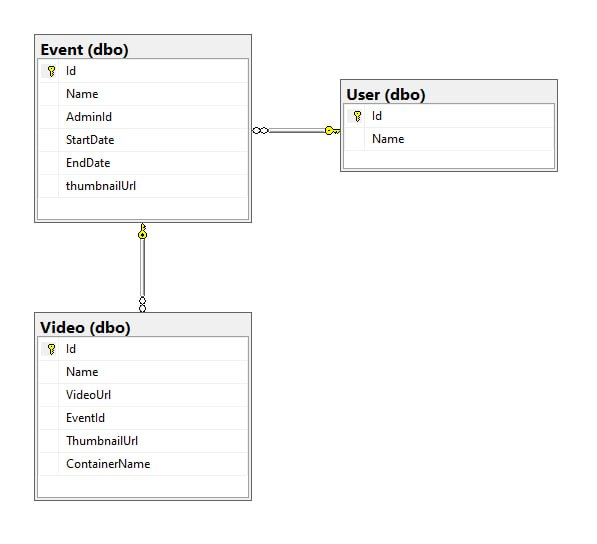
\includegraphics[scale=0.5]{diagrammi/database.png} 
    \caption{Diagramma del database}
    \label{fig:schema database}
\end{figure}

\pagebreak

\section{Progettazione del frontend}
La progettazione del frontend è sviluppata sulla base dell'utilizzo di React come libreria principale per lo sviluppo dell'interfaccia utente.
%  Verranno illustrati i principi di progettazione di React, come la creazione di componenti riutilizzabili, la gestione dello stato dell'applicazione e la definizione delle rotte per la navigazione. Saranno presentati anche i diagrammi dell'architettura del frontend, mostrando come i componenti si integrano per creare un'esperienza utente coerente.
\subsection{Architettura del frontend}
Il frontend è sviluppato utilizzando un template disposto dall'azienda, che utilizza il design pattern Container-Presenter, è composto da due componenti principali: il Container e il Presenter.
Il primo è responsabile della gestione dello stato dell'applicazione, dell'interazione con i dati e della logica di business, si occupa di recuperare i dati, gestire gli eventi, effettuare chiamate API e gestire lo stato globale dell'applicazione; il secondo invece, è responsabile dell'aspetto visuale e dell'interfaccia utente, riceve i dati e le funzioni dai Container e si occupa di renderizzare l'interfaccia utente in base ai dati ricevuti.\\
La comunicazione tra i due avviene tramite le props, in quanto il Container passa i dati al Presenter tramite props, mentre il Presenter invia le informazioni tramite callback fornite dal Container.\\
Lo schema rappresentativo dell'architettura è presente nella figura \ref{fig:Diagrammafrontend}.
\begin{figure}[!h] 
    \centering 
    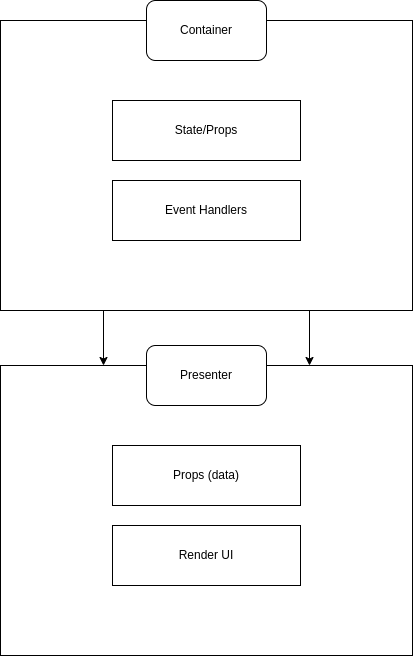
\includegraphics[scale=0.5]{diagrammi/frontend.drawio.png} 
    \caption{Diagramma design pattern Container-Presenter}
    \label{fig:Diagrammafrontend}
\end{figure}
\clearpage
\section{Progettazione del backend}
La progettazione del backend è sviluppata sulla base dell'utilizzo del linguaggio di programmazione C\texttt{\#} e del framework ASP.NET Core.\\
\subsection{Architettura del backend}
Il backend è sviluppato utilizzando un template disposto dall'azienda, che utilizza una separazione delle componenti in layer distinti, dove ognuno ha un compito specifico.\\
Il template è composto da tre layer fondamentali: API, Core e Data; il primo è responsabile della comunicazione con il frontend, il secondo è responsabile della gestione dello stato dell'applicazione e il terzo è responsabile della comunicazione con il database.\\
Lo schema rappresentativo dell'architettura è presente nella figura \ref{fig:Diagrammabackend}.
\begin{figure}[H] 
    \centering 
    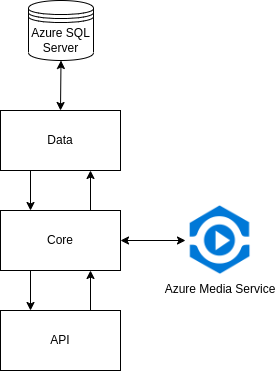
\includegraphics[scale=0.5]{diagrammi/backend.png} 
    \caption{Diagramma architettura del backend}
    \label{fig:Diagrammabackend}
\end{figure}
\subsubsection{API}
È responsabile della comunicazione con il frontend, è composto da due parti: i controller e i \gls{DTO}. Il primo ha il compito di gestire le richieste HTTP provenienti dal frontend e coordinare le azioni richieste per soddisfarle: quando un controller riceve una richiesta, estrae i dati necessari dalla richiesta e interagisce con i layer Core per fornire una risposta al Client. 
Il secondo ha il compito di definire la struttura dei dati che vengono trasferiti tra il frontend e il backend durante la chiamata, in modo da consentire una comunicazione standardizzata e senza ambiguità. I DTO possono includere solo i campi necessari per soddisfare una certa richiesta, così facendo, riducono il trasferimento di dati inutili e rendono la comunicazione più veloce; oltre a ciò, sono utilizzati anche per la validazione dei dati, garantendo che i dati ricevuti dal frontend siano validi.\\
\subsubsection{Core}
Il layer Core è responsabile della gestione dello stato dell'applicazione. Riceve le richieste dal layer API e le elabora, interagendo con il layer Data per ottenere i dati necessari; è composto da due parti: i models e i service. I models rappresentano la struttura dei dati che vengono utilizzati dall'applicazione per effettuare le operazioni richieste; i service, invece, gestiscono la logica dell'applicazione, contengono i metodi che vengono chiamati dai controller, che eseguono operazioni con i servizi esterni e con il layer Data.\\
\subsubsection{Data}
Il layer Data è responsabile dell'accesso ai dati, è composto da tre parti: Context, Entity e Provider. Il primo ha il compito di gestire la connessione con il database, definisce la struttura del database e fornisce i metodi per accedervi; il secondo ha il compito di definire la struttura dei dati che vengono salvati nel database; il terzo ha il compito di gestire la comunicazione con il database, fornisce i metodi per accedere ai dati per effettuare le operazioni di lettura e scrittura.\\

\section{Integrazione con Azure}
Azure è una piattaforma cloud proprietaria di Microsoft che offre vari servizi.
La WebApp è integrata con Azure per la gestione del database, gestione dei video e per la distribuzione dell'applicazione, sono utilizzati i seguenti servizi: SQL Server, Azure Media Service e Azure App Service.\\
\subsection{Azure SQL Server}
Il progetto integra un database SQL ospitato su Azure SQL Server, che permette di gestire il database in maniera semplice e veloce, senza dover gestire l'infrastruttura. Il collegamento al database è gestito dal layer Data del backend, che utilizza Entity Framework Core per la gestione del database.\\
\subsection{Azure Media Service}
Il progetto utilizza Azure Media Service per la gestione dei video, in particolare per la codifica, l'archiviazione e la distribuzione dei video. Il collegamento ad Azure Media Service è gestito dal layer Core del backend, che utilizza il package NuGet Microsoft.Azure.Management.Media per la gestione dei video.\\
\subsubsection{Codifica}
Per lo sviluppo di questo PoC è stato deciso di codificare i video in H.264 e utilizzando il preset Adaptive Streaming, che permette di codificare il video in diversi formati e risoluzioni, in modo da adattarsi alla qualità della rete e al dispositivo utilizzato. Sono state scelte queste impostazioni che permettono di ottenere un video di risoluzione massima pari a 1080p.\\
\subsubsection{Archiviazione}
Quando un video termina la codifica, viene archiviato in un container di Azure Media Service, che permette il salvataggio dei vari file video, della thumbnail, dei metadati e del manifest.\\
\subsubsection{Distribuzione}
Una volta archiviato, il video viene distribuito tramite Streaming Endpoint, che creano un Url al manifest del video e all'immagine di thumbnail, che vengono poi salvati nel database tramite apposite API.\\
\subsubsection{Azure App Service}
Sia il modulo FrontEnd che il modulo del Backend vengono distribuiti attraverso Azure App Service, vengono inizializzati tramite l'apposita funzione di Visual Studio 2022.\\ 
    \chapter{Implementazione}
\label{cap:implementazione}

L'implementazione del PoC è una parte fondamentale del progetto di stage, in quanto permette di verificare la fattibilità del prodotto e di valutare la bontà delle scelte progettuali.\\
In questo capitolo verranno descritte le principali scelte implementative, sia per quanto riguarda il frontend che il backend.\\

\section{Struttura del progetto}
La struttura del progetto è stata organizzata in modo da separare il frontend dal backend, in modo da poterli sviluppare in modo indipendente. Inoltre, è stato scelto di utilizzare una repository su Azure DevOps per il versioning del codice, in modo da poter avere una storicizzazione delle modifiche.
\section{Backend}
Il backend è stato sviluppato utilizzando il linguaggio di programmazione C\texttt{\#} e il framework ASP.NET Core, è basato sul template fornito dall'azienda che prevede l'utilizzo di un'architettura a layer.\\
Come ambiente di sviluppo è stato utilizzato Visual Studio 2022.\\
\subsection{Architettura a layer}
L'architettura a layer è una tipologia di architettura software che prevede la suddivisione del codice in diversi livelli, ognuno dei quali ha un compito ben preciso, e che comunica con gli altri livelli attraverso interfacce. Questo permette di avere un codice più modulare e mantenibile, in quanto ogni livello ha un compito ben preciso e non si occupa di altro.\\
Il backend è composto da un unico progetto "AdMaioraStreamingPOC", che contiene i vari layer suddivisi in cartelle, ognuna delle quali contiene le soluzioni relative al layer. I layer sono: API, Core e Data.\\

\subsubsection{API}
Il layer API è il livello più esterno dell'applicazione, si occupa di gestire le richieste HTTP in arrivo dal frontend. È divisa in due soluzioni: Controller e DTO.\\
\begin{itemize}
    \item \textbf{Controllers}: sono le classi che si occupano di gestire le richieste HTTP in arrivo dal frontend, utilizzano il framework ASP.NET Core e la libreria AutoMapper per la conversione dei DTO in entità e viceversa; inoltre, utilizzano la dependency injection per iniettare le dipendenze necessarie dalle classi di Service presenti nel layer Core, l'uso di questa tecnica rende i controller indipendenti dalle implementazioni concrete delle dipendenze.\\
    Per ogni entità del database è stato creato un controller, che contiene metodi CRUD e non, per gestire le richieste HTTP in modo completo. Quando un controller riceve una richiesta HTTP, utilizza i metodi presenti nel Service per gestire la richiesta, e restituisce al frontend il risultato della richiesta in formato JSON.\\
    \item \textbf{DTO}: sono classi che contengono la struttura dei dati che vengono scambiati tra il frontend e il backend.
    Per ogni entità del database sono stati creati tre DTO: uno per la creazione, uno per l'aggiornamento e uno per la visualizzazione; così facendo, si evita di scambiare dati inutili tra frontend e backend, e si evita di dover gestire la serializzazione e deserializzazione di dati inutili. Inoltre, utilizzando i DTO, si evita di dover esporre le entità del database al frontend, favorendo la separazione tra frontend e backend.\\
\end{itemize}
\subsubsection{Core}
Il layer Core è il livello intermedio dell'applicazione, e si occupa di gestire la logica di business dell'applicazione. È diviso in due soluzioni: Model e Services.\\
\begin{itemize}
    \item \textbf{Model}: sono classi che rappresentano le entità nel database, il loro scopo è quello di mappare le entità del database in classi C\texttt{\#}, in modo da poterle utilizzare all'interno della logica del codice. Per ogni entità del database è stato creato un Model, che contiene le proprietà dell'entità.\\
    \item \textbf{Services}: sono classi che si occupano di gestire la logica di business dell'applicazione, utilizzano i Model per accedere ai dati nel database, e li restituiscono al layer API. Per ogni entità del database è stato creato un Service, che contiene  metodi CRUD e non, per gestire la logica di business dell'applicazione. Fornisce i metodi al layer API attraverso interfacce, inoltre vengono iniettate le dipendenze necessarie del Provider presente nel layer Data, le credenziali per l'accesso ad Azure e della configurazione per il server TUS.io. Il suo scopo principale è quello di fornire un'interfaccia tra il layer API e il layer Data. Inoltre si occupa anche della comunicazione con i servizi esterni, infatti gestisce l'upload dei video su Azure Media Services, tramite le sue API dedicate e comunica con l'istanza TUS.io.\\
\end{itemize}
\subsubsection{Data}
Il layer Data è il livello più interno dell'applicazione, e si occupa di gestire l'accesso ai dati nel database. È diviso in tre soluzioni: Context, Providers e Entity.\\
\begin{itemize}
\item \textbf{Context}: è la classe che si occupa di gestire l'accesso ai dati nel database, che quando viene inizializzato, gli viene iniettata la configurazione per il collegamento e definisce tre proprietà di tipo DbSet, una per ogni entità del database, che consentono di effettuare operazione di query e manipolazione dei dati.\\
\item \textbf{Providers}: sono classi che si occupano di gestire l'accesso ai dati nel database, utilizzando il Context per accedervi, e li restituiscono al layer Core convertendoli in Model tramite AutoMapper. È stata creata una classe per ogni entità del database, e contengono i metodi CRUD per gestire l'accesso ai dati nel database. Lo scopo principale dei providers è quindi quello di fornire un'interfaccia tra il layer Core e il database.\\
\item \textbf{Entity}: sono classi che rappresentano le entità nel database, il loro scopo è quello di mappare le entità del database in classi C\texttt{\#}, in modo da poterle utilizzare all'interno della logica del codice. Per ogni entità del database è stato creato un Entity, che contiene le proprietà dell'entità. Queste classi sono utilizzate dal Context per accedere ai dati nel database. Oltre a ciò, vengono utilizzate per definire le proprietà, tramite il framework Entity Framework Core e il suo sistema di migrazioni: quando viene modificata una proprietà di un Entity, viene eseguita una migrazione che modifica la struttura del database in base alle modifiche apportate.\\
\end{itemize}
\section{Frontend}
Il frontend è stato sviluppato utilizzando il framework React e la libreria grafica Material-UI.\\
Il frontend è diviso in tre cartelle principali: Components, Pages e Services, utilizzando il template fornito dall'azienda che prevede l'utilizzo del template Container-Presenter.\\
È stato utilizzato Visual Studio code come ambiente di sviluppo, e Node.js come runtime per l'esecuzione del codice.\\

\subsection{Architettura}
L'architettura del frontend è divisa in tre cartelle: Pages, Common e Context.

\subsubsection{Pages}
La cartella Pages contiene le pagine dell'applicazione, ovvero le pagine che vengono visualizzate dall'utente. Ogni pagina è divisa a sua volta in tre componenti: Context, Page e Components.\\

\begin{itemize}
    \item \textbf{Context}: svolge il ruolo di fornire un meccanismo per l'accesso e la condivisione dei dati tra i componenti, in modo da evitare di dover passare i dati da un componente all'altro. Per ogni pagina è stato creato un Context, che contiene un provider che contiene lo stato e le funzioni per l'accesso ai dati; ogni componente avvolto dal provider può accedere ai dati e alle funzioni per modificarli. L'accesso ai dati avviene tramite l'utilizzo del context di FetchContext, che contiene le route per effettuare le chiamate al backend.\\
    \item \textbf{Page}: Ogni pagina contiene un componente PageContent, che renderizza i componenti della pagina. Successivamente essi vengono avvolti dal Provider della pagina specifica che permette l'accesso al Context della pagina, in modo tale che possano accedere ai dati e alle funzioni per modificarli.\\
    \item \textbf{Components}: sono le porzioni di codice che vengono renderizzate all'interno della pagina.
\end{itemize}
\subsubsection{Common}
La cartella Common contiene i componenti che vengono utilizzati in tutte le pagine, è composto da tre file:
\begin{itemize}
    \item \textbf{Layout}:definisce la struttura di ogni pagina, composta a sinistra da un menù laterale, sopra dal titolo della pagina corrente e al centro dal contenuto della pagina passato come props.
    Il menù laterale è composto da una lista di MenuItems, che vengono renderizzati grazie all'utilizzo del context di NavContext.
    \item \textbf{Route}: permette di navigare tra le pagine in base al percorso specificato contenuto nel MenuItems.\\
    \item \textbf{DialogCustom}: è un componente che permette di visualizzare un dialog, che contiene un titolo, un contenuto e due bottoni, uno per confermare e uno per annullare. Viene utilizzato in tutte le pagine per confermare le azioni che possono modificare i dati nel database. Il contenuto viene passato tramite props, in modo da poterlo personalizzare in base alla pagina. L'utilizzo di questo componente permette di evitare di dover creare un dialog pressoché identico in tutte le pagine.\\
\end{itemize}
\subsubsection{Context}
La cartella Context, contiene i file di contesto, è composta da tre file: FetchContext, NavContext e ToastContext.
\begin{itemize}
    \item \textbf{FetchContext}: contiene le route per effettuare le chiamate al backend, è composto da una funzione "Compile Route" che permette di comporre la route in base ai parametri passati, e da una funzione "Fetch" che permette di effettuare la chiamata al backend. Questo permette di evitare di dover ripetere le route in ogni componente.\\
    \item \textbf{NavContext}: contiene le route per effettuare la navigazione tra le pagine, è composto da vari metodi per per la navigazione, per la gestione del menù laterale, per la gestione del titolo della pagina e per la gestione del breadcrumb. \\
    \item \textbf{ToastContext}: contiene le funzioni per mostrare i toast, composto da quattro funzioni: "Success", "Error", "Warning" e "Info", che permettono di mostrare un toast con il messaggio passato come parametro.\\
\end{itemize}
\subsection{Interfaccia grafica}
\subsubsection{Pagina Home}
La pagina Home è la pagina principale dell'applicazione, contiene una grid di tutti gli eventi disponibili, e un menù laterale che permette la navigazione tra le pagine.\\
In figura \ref{fig:home} è rappresentano un esempio della pagina home sviluppata.
\begin{figure}[H]
    \centering
    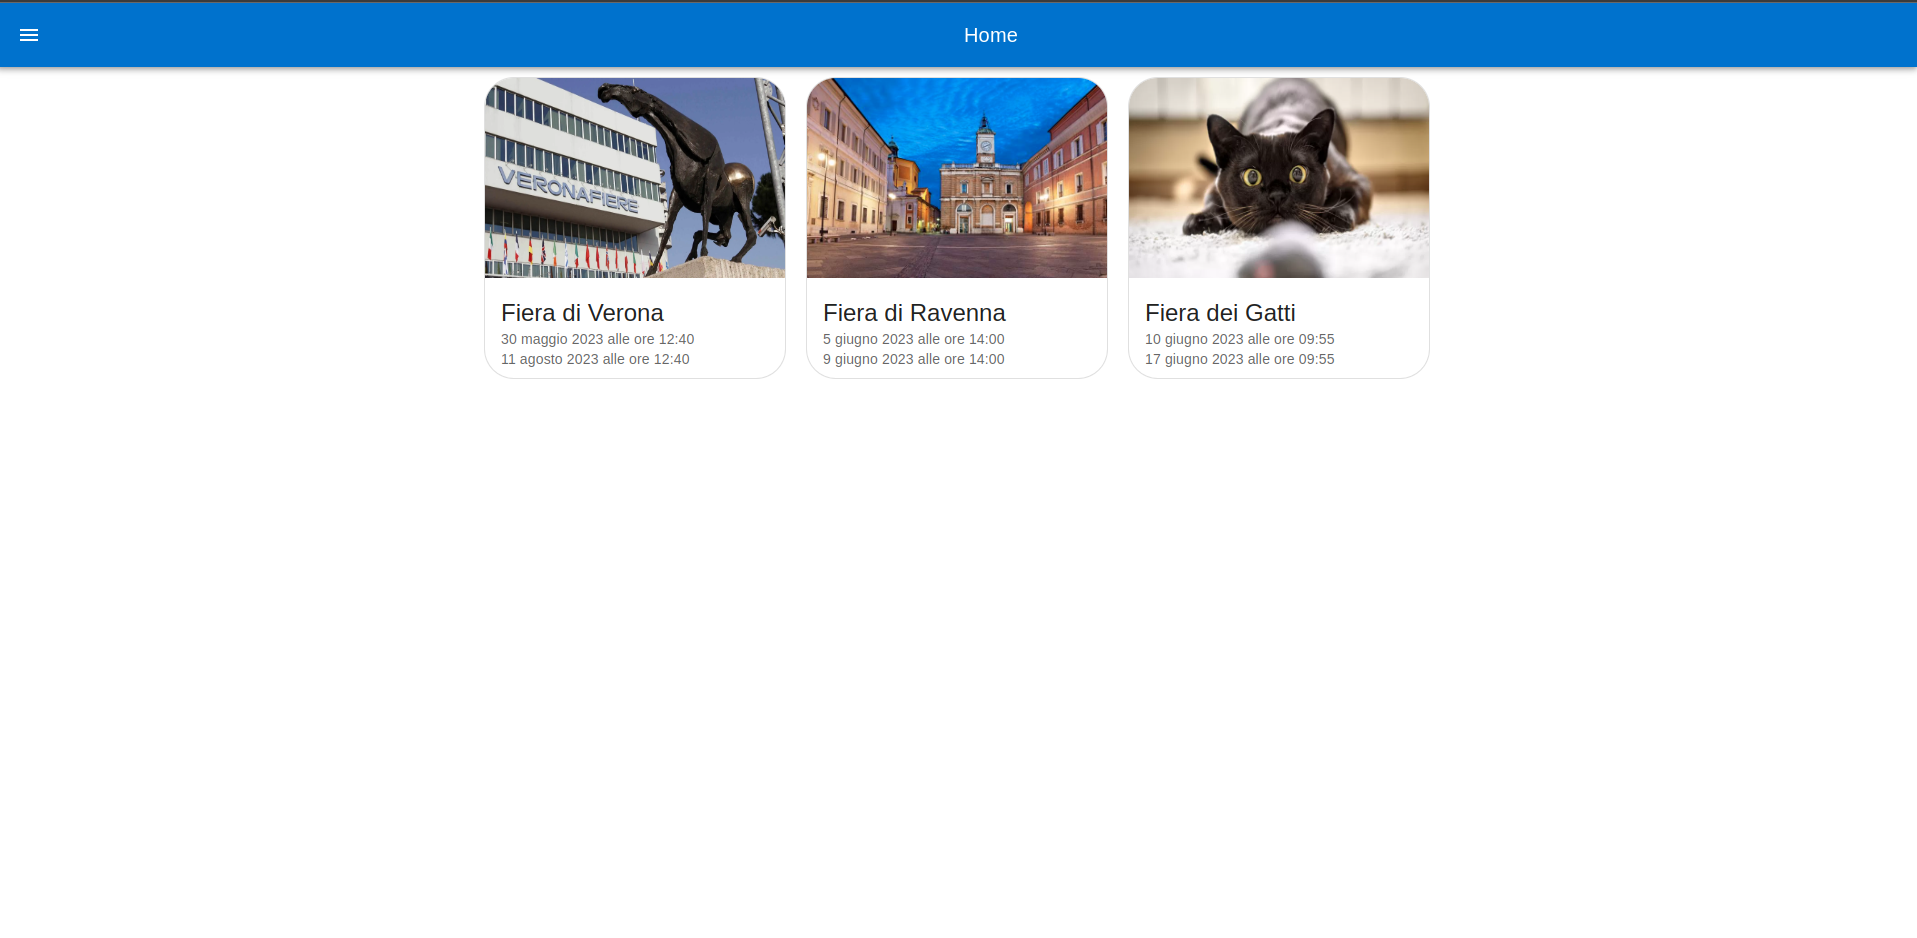
\includegraphics[width=1\textwidth]{images/interface/home.png}
    \caption{Pagina Home}
    \label{fig:home}
\end{figure}
\subsubsection{Pagina Eventi}
Quando si clicca su un evento nella pagina Home, si viene reindirizzati alla pagina dell'evento, che contiene una grid con tutti i video dell'evento.\\
In figura \ref{fig:eventi} è rappresentano un esempio della pagina di un evento inserito nel sistema.
\begin{figure}[H]
    \centering
    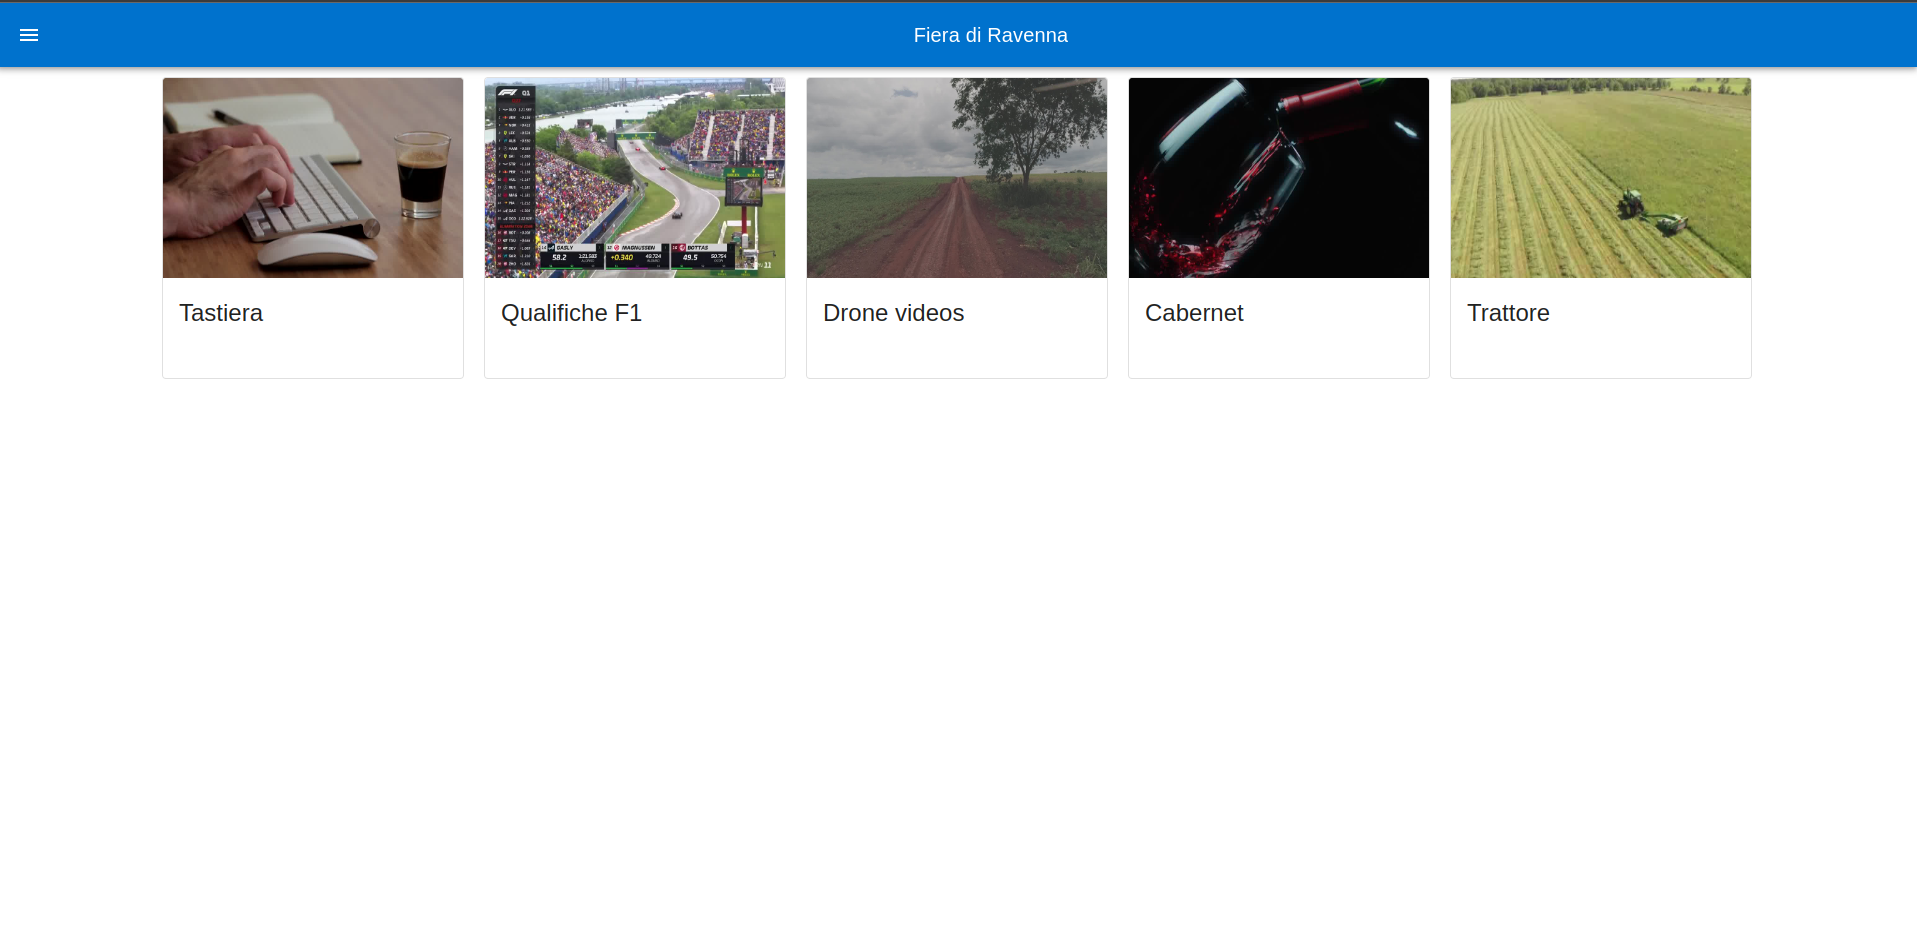
\includegraphics[width=1\textwidth]{images/interface/events.png}
    \caption{Pagina Eventi}
    \label{fig:eventi}
\end{figure}
\subsubsection{Pagina Video}
Quando si clicca su un video nella pagina Eventi, si viene reindirizzati alla pagina del video, che contiene il player del video e i pulsanti per la gestione.\\
In figura \ref{fig:video} è rappresentano un esempio di visualizzazione di un video.
\begin{figure}[H]
    \centering
    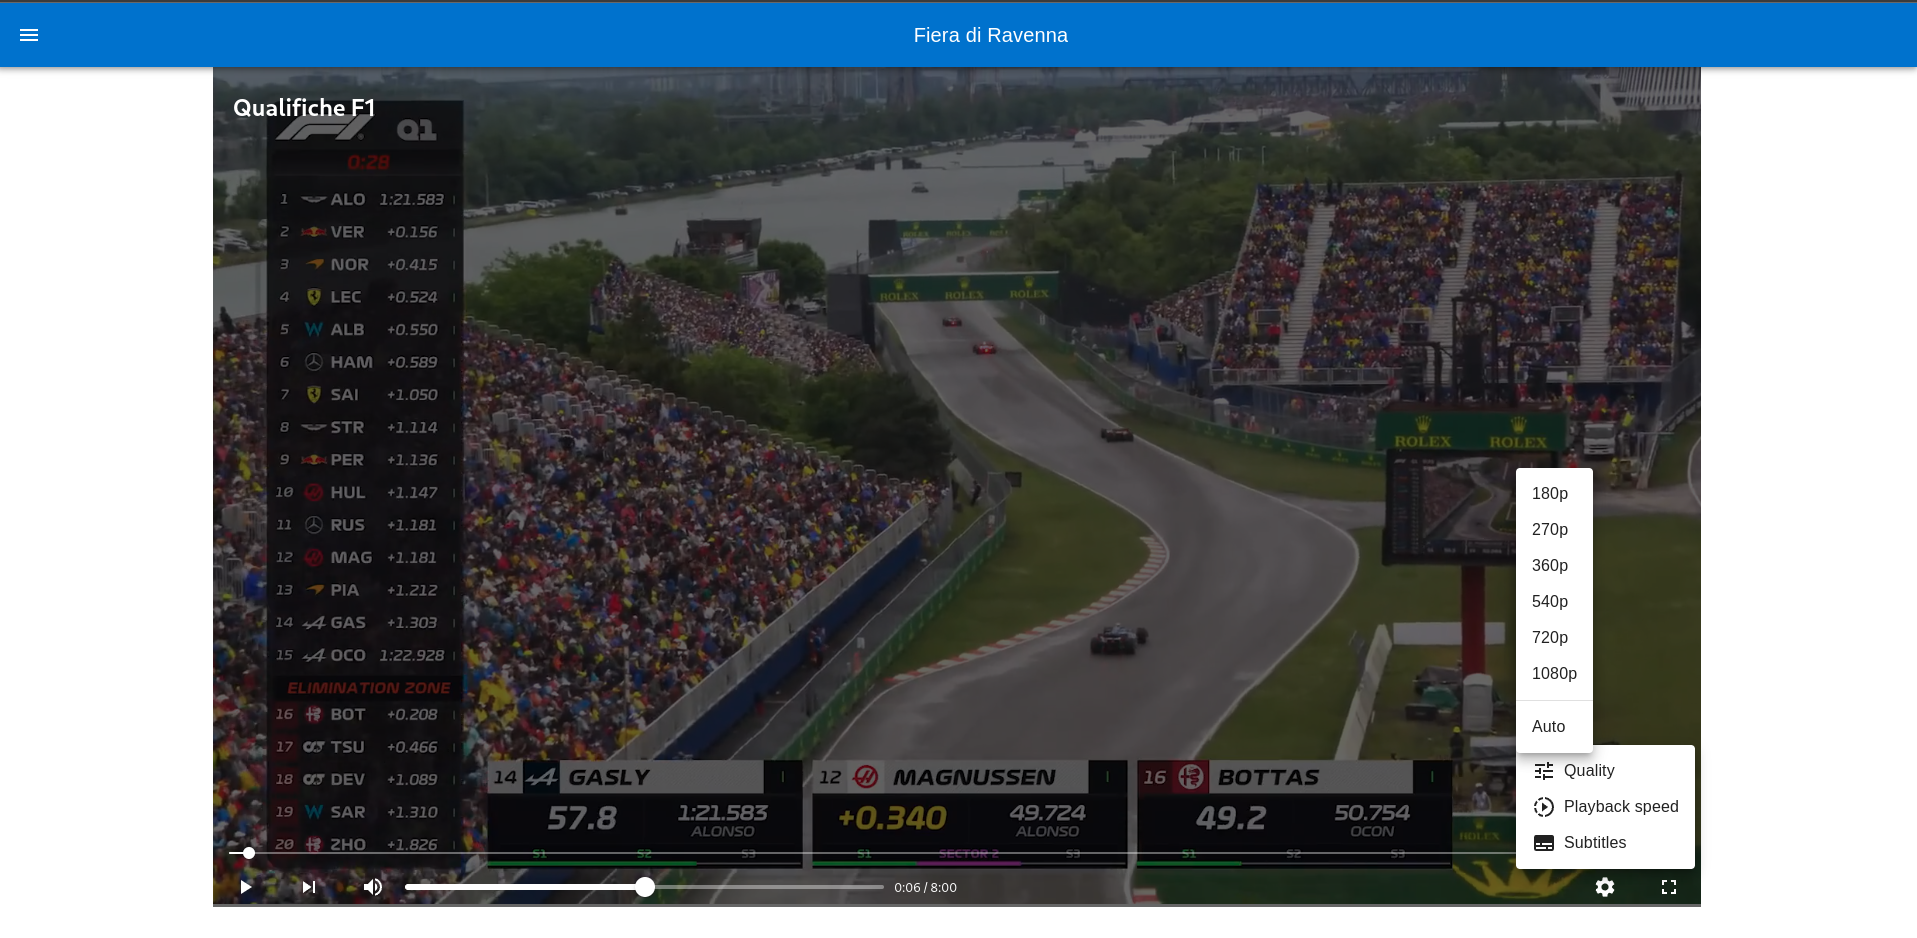
\includegraphics[width=1\textwidth]{images/interface/video.png}
    \caption{Pagina Video}
    \label{fig:video}
\end{figure}
\subsubsection{Pagina Gestione}
Le pagine di gestione sono tre, una per gli eventi, una per i video e una per gli utenti. Ogni pagina contiene una tabella con tutti gli elementi, ogni riga contiene due pulsanti, uno per modificare l'elemento e uno per eliminarlo. Inoltre è presente anche un pulsante per aggiungere un nuovo elemento attraverso un dialog.\\
In figura \ref{fig:gestionevideo} è rappresentana la pagina della tabella per la gestione dei video.
\begin{figure}[H]
    \centering
    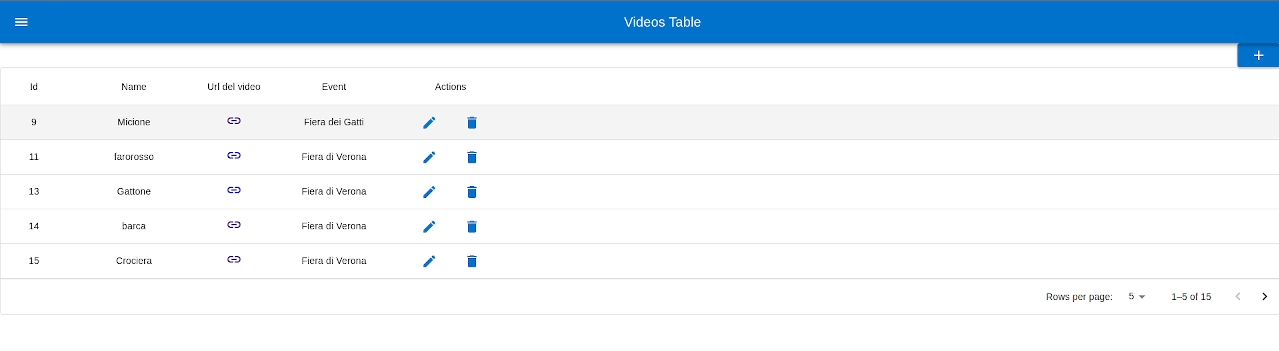
\includegraphics[width=1\textwidth]{images/interface/videotable.png}
    \caption{Pagina Gestione dei video}
    \label{fig:gestionevideo}
\end{figure}
Quando viene premuta l'icona della matita, si apre un dialog, come in figura \ref{fig:modifica video}, tramite la quale l'utente può modificare i dati del video.
\begin{figure}[H]
    \centering
    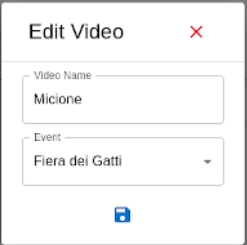
\includegraphics[width=0.3\textwidth]{images/interface/editvideo.png}
    \caption{Dialog Modifica Video}
    \label{fig:modifica video}
\end{figure}
Quando viene premuto il bottone di aggiunta, si apre un dialog, come in figura \ref{fig:aggiuntavideo}, tramite il quale l'utente può selezionare un video da caricare e i dati relativi ad esso.
\begin{figure}[H]
    \centering
    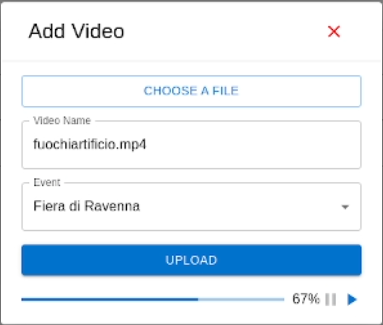
\includegraphics[width=0.3\textwidth]{images/interface/addvideo.png}
    \caption{Dialog Aggiunta Video}
    \label{fig:aggiuntavideo}
\end{figure}
\section{Integrazione con Azure}
Per l'integrazione con i servizi di Azure, sono state utilizzate le API ufficiali fornite da Microsoft, che permettono di gestire i servizi di Azure in modo semplice e veloce.\\
La connessione al database è stata gestita mediante l'utilizzo del framework Entity Framework Core; quando il programma viene inizializzato, nel backend al livello del provider viene iniettata la configurazione per il collegamento al database, che contiene le credenziali per l'accesso al database. Per quanto riguarda il collegamento con Azure Media Service, e vengono utilizzate nel backend nel layer Service per comunicare con le API proprietarie.

\section{Integrazione con TUS.io}
Per la gestione dell'upload dei video dal frontend al backend, è stato utilizzato il servizio TUS.io, che permette di gestire l'upload di file di grandi dimensioni e di gestirne lo stato. Quando viene inizializzato il programma, viene creata un'istanza del server TUS.io, che permette al frontend tramite le API di accedere ad esso e di gestire l'upload dei file. Quando un file viene caricato sul server TUS.io, il frontend invia una chiamata al backend con l'id TUS del file caricato e poi viene passato ai metodi del Service, che si occupa di recuperare il file e successivamente di caricarlo su Azure Media Services.\\

    \chapter{Testing e validazione}
\intro{In questo capitolo verranno descritte le attività di testing e validazione svolte sul POC.}\\
\section{Descrizione delle attività di testing}

\section{Verifica dei requisiti}

\section{Analisi dei risultati}

\section{Valutazione delle prestazioni della webapp}
    \chapter{Analisi dei costi}
\label{cap:analisi-costi}
\intro{In questo capitolo verrà descritta l'analisi dei costi effettuata sul progetto.}\\

\section{Introduzione}
\label{sec:introduzione}
L'analisi dei costi è un'attività fondamentale per la realizzazione di un progetto, in quanto permette di stimare il costo totale del progetto e di conseguenza il budget necessario per la sua realizzazione e mantenimento.\\
Verranno descritti i principali costi di mantenimento della WebApp, in particolare verranno analizzati i costi di hosting, di distribuzione e caricamento dei video, che essendo basata sull'utilizzo del infrastruttura di Azure, sono i costi principali.\\

\subsection{Costi di hosting}
\label{subsec:costi-hosting}
I costi di hosting sono i costi necessari per mantenere la WebApp online, in particolare sono i costi per l'hosting del backend e del frontend. Durante lo sviluppo del PoC, è stato utilizzato un piano di distribuzione gratuito, che permette di distribuire l'applicazione senza costi aggiuntivi con delle limitazioni sulle operazioni che possono essere effettuate. In caso di produzione dell'applicazione, è necessario considerare dei costi per l'hosting, in quanto il piano gratuito non è adatto per l'hosting di un'applicazione in produzione. Azure offre diversi piani di hosting, che differiscono per le risorse disponibili e per il costo. Il piano piu adatto per una WebApp di questo tipo in produzione è il piano Premium, che offre un numero illimitato di App, 250GB di spazio di archiviazione, fino a 30 istanze e la possibilità di utilizzare un dominio personalizzato e l'autoscale ad un costo di 0.184€/h, ovvero 4.416€/giorno.\\
\subsection{Costi di codifica}
I costi di codifica sono i costi necessari per effettuare la codifica dei video caricati nei vari formati, sono riportati nella seguente tabella //TODO: link alla tabella.
Per lo sviluppo del PoC è stata utilizzata la codifica in HD, idealmente per l'app in produzione si utilizzerà la codifica in 4K visto l'evoluzione della disponibilità di rete e dell'aumento delle risoluzioni dei dispositivi sempre più accessibili.

\subsection{Costi di trasferimento}
Azure Media Service prevede un costo fisso per ogni GB trasferito tra le stesse zone di distribuzione, ovvero che se il file richiesto si trova in Europa e anche il richiedente avrà un costo di 0.010€/GB mentre se si trovano in zone differenti i costi aumentano come riportato nella seguente tabella //TODO: link alla tabella

\subsection{Costi di distribuzione}
\label{subsec:costi-distribuzione}
I costi di distribuzione sono i costi necessari per la distribuzione in streaming dei contenuti multimediali. Durante lo sviluppo del PoC è stato utilizzato lo Standard Streaming Endpoint, che ha un Bandwidth di 600Mbps a un costo di 1.9088€/giorno, ovvero 59.172€/mese, che è il piano più basso disponibile, permette una distribuzione a circa 171 utenti contemporaneamente con un utilizzo medio di 3.5Mbps per utente. È limitante in quanto, una volta saturato il Bandwidth, non permette la scalabilità automatica, che causerebbe buffering ai client, e bisognerebbe passare ad un piano superiore.\\

\section{Consuntivo preventivato}
In caso di produzione dell'applicazione, è necessario stimare il numero di utenti che utilizzeranno l'applicazione per poter scegliere i piani più adatti e avere una stima dei costi circa accurata.\\
È stato realizzato un modello matematico che stima in base ai dati messi in input come numero di utenti iscritti, percentuale di utenti attivi giornalmente, durata media di visione per utente, orari e ampiezza del picco, qualità video richiesta, il costo medio giornaliero dell'applicazione, che prevede i costi di codifica, trasferimento e distribuzione, vengono riportati tre scenari.
Per congruenza dei dati, ogni scenario prevede gli stessi dati in input tranne che per il numero di iscritti:

\begin{table}[H]
    \label{tab:dati-input}
    \begin{tabularx}{\textwidth}{|c|X|}
        \hline
        \textbf{Oggetto} & \textbf{Valore} \\\hline
        
        \textbf{Percentuale utenti iscritti} & {10\%} \\ 
        \hline
        \textbf{Durata media visualizzazioni in secondi} & {300s} \\ 
        \hline
        \textbf{Percentuale richieste HD} & {50\%}\\
        \hline
        \textbf{Percentuale richieste FHD} & {50\%}\\  
        \hline
        \textbf{Banda media HD} & {4Mbps}\\  
        \hline
        \textbf{Banda media FHD} & {7Mbps}\\  
        \hline
        \textbf{Costo per singolo Premium Unit Streaming} & {0.17€}\\  
        \hline
        \textbf{Costo per GB trasferito} & {0.010€}\\  
        \hline
    \end{tabularx}
    \caption{Tabella di dati in input}

\end{table}

\subsubsection{Caso 10000 utenti iscritti}
Per il primo scenario, si è scelto di considerare 10000 utenti iscritti, che è un numero ragionevole per una WebApp di questo tipo all'inizio della sua vita.\\
\begin{table}[H]
    \label{tab:costi-10000}
    \begin{tabularx}{\textwidth}{|c|X|}
        \hline
        \textbf{Oggetto} & \textbf{Valore} \\\hline
        
        \textbf{Costo App Service Giornaliero} & {4.416€} \\ 
        \hline
        \textbf{GB usati giornalmente} & {201 GB} \\ 
        \hline
        \textbf{Costo di trasferimento} & {2.014€}\\
        \hline
        \textbf{Costo totale di Premium Unit Streaming} & {4.17€}\\  
        \hline
        \textbf{Totale giornaliero} & {10.60€}\\  
        \hline
        \textbf{Totale mensile} & {328.45€}\\  
        \hline
        \textbf{Totale annuale} & {3.867.23€}\\  
        \hline
    \end{tabularx}
    \caption{Tabella costi con 10000 utenti iscritti}
\end{table}
\begin{figure}[H]
    \centering
    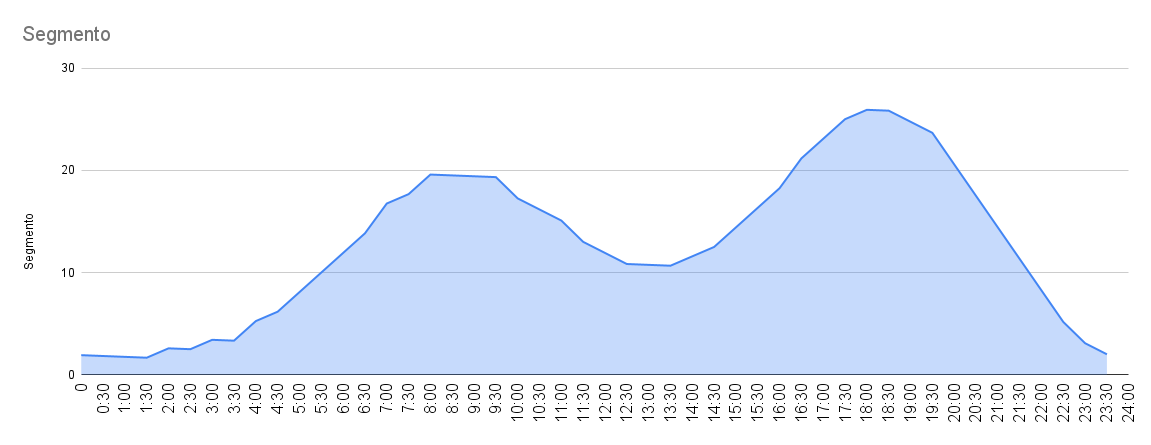
\includegraphics[scale=0.25]{images/costi/10kuser.png}
    \caption{Grafico utenti/orario con 10000 utenti iscritti}
    \label{fig:costi-10000}
\end{figure}
\subsubsection{Caso 100000 utenti iscritti}
Per il secondo scenario, si è scelto di considerare 100000 utenti iscritti, che è un buon numero di utenti per una WebApp di questo tipo in caso iniziasse a crescere.\\
\begin{table}[H]
    \label{tab:costi-100000}
    \begin{tabularx}{\textwidth}{|c|X|}
        \hline
        \textbf{Oggetto} & \textbf{Valore} \\\hline
        
        \textbf{Costo App Service Giornaliero} & {4.416€} \\ 
        \hline
        \textbf{GB usati giornalmente} & {2014 GB} \\ 
        \hline
        \textbf{Costo di trasferimento} & {20.142€}\\
        \hline
        \textbf{Costo totale di Premium Unit Streaming} & {7.02€}\\  
        \hline
        \textbf{Totale giornaliero} & {31.57€}\\  
        \hline
        \textbf{Totale mensile} & {978.80€}\\  
        \hline
        \textbf{Totale annuale} & {11524.64€}\\  
        \hline
    \end{tabularx}
    \caption{Tabella costi con 100000 utenti iscritti}
\end{table}
\begin{figure}[H]
    \centering
    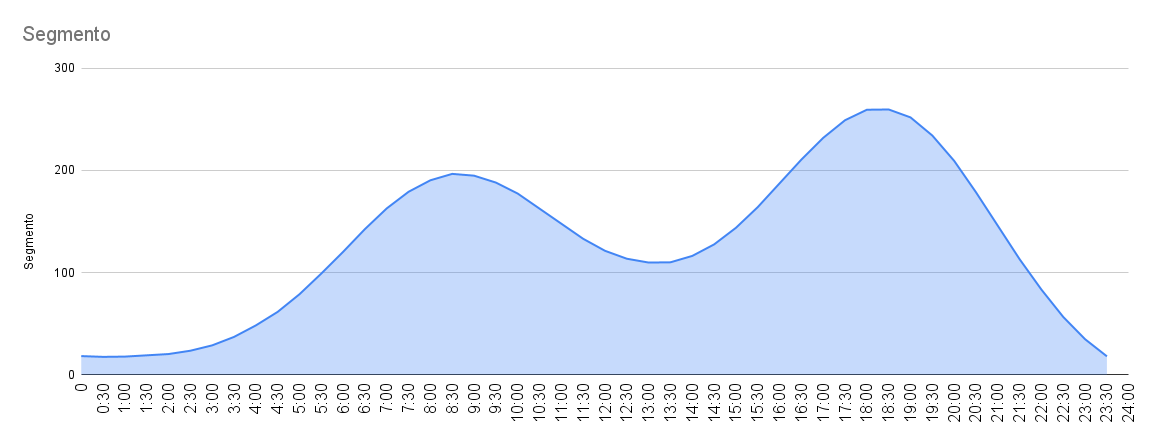
\includegraphics[scale=0.25]{images/costi/100kuser.png}
    \caption{Grafico utenti/orario con 100000 utenti iscritti}
    \label{fig:costi-100000}
\end{figure}

\subsubsection{Caso 1000000 utenti iscritti}
Per il terzo scenario, si è scelto di considerare 1000000 utenti iscritti, che è un numero importante di utenti in caso la WebApp avesse un grande successo.\\
\begin{table}[H]
    \label{tab:costi-1000000}
    \begin{tabularx}{\textwidth}{|c|X|}
        \hline
        \textbf{Oggetto} & \textbf{Valore} \\\hline
        
        \textbf{Costo App Service Giornaliero} & {4.416€} \\ 
        \hline
        \textbf{GB usati giornalmente} & {20142 GB} \\ 
        \hline
        \textbf{Costo di trasferimento} & {201.416€}\\
        \hline
        \textbf{Costo totale di Premium Unit Streaming} & {11.13€}\\  
        \hline
        \textbf{Totale giornaliero} & {216.96€}\\  
        \hline
        \textbf{Totale mensile} & {6725.85€}\\  
        \hline
        \textbf{Totale annuale} & {79191.41€}\\  
        \hline
    \end{tabularx}
    \caption{Tabella costi con 1000000 utenti iscritti}
\end{table}
\begin{figure}[H]
    \centering
    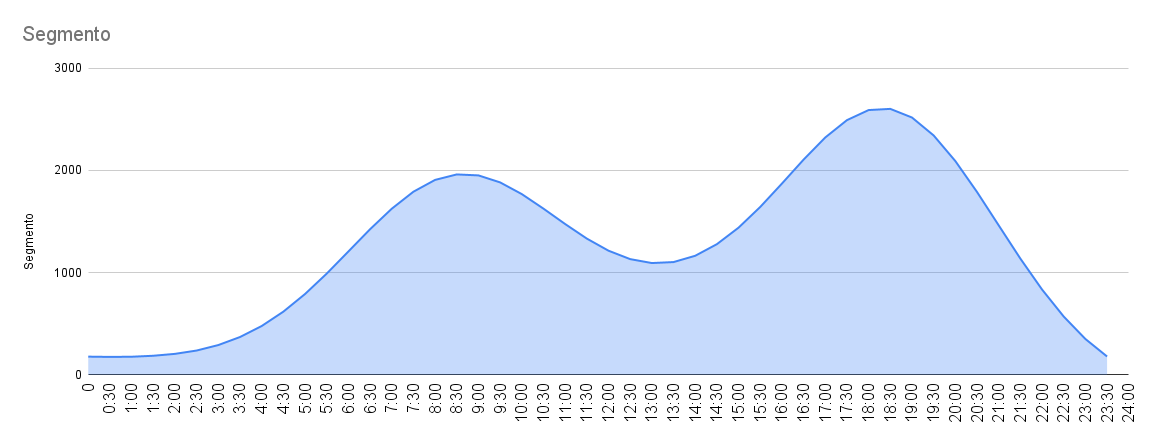
\includegraphics[scale=0.25]{images/costi/1000kuser.png}
    \caption{Grafico utenti/orario con 1000000 utenti iscritti}
    \label{fig:costi-1000000}
\end{figure}
    % \chapter{Descrizione dello stage}
\label{cap:descrizione-stage}

\intro{Breve introduzione al capitolo}\\

\section{Introduzione al progetto}

\section{Analisi preventiva dei rischi}

Durante la fase di analisi iniziale sono stati individuati alcuni possibili rischi a cui si potrà andare incontro.
Si è quindi proceduto a elaborare delle possibili soluzioni per far fronte a tali rischi.\\

\begin{risk}{Performance del simulatore hardware}
    \riskdescription{le performance del simulatore hardware e la comunicazione con questo potrebbero risultare lenti o non abbastanza buoni da causare il fallimento dei test}
    \risksolution{coinvolgimento del responsabile a capo del progetto relativo il simulatore hardware}
    \label{risk:hardware-simulator} 
\end{risk}

\section{Requisiti e obiettivi}


\section{Pianificazione}

    % \chapter{Analisi dei requisiti}
\label{cap:analisi-requisiti}

\intro{Breve introduzione al capitolo}\\

\section{Casi d'uso}

Per lo studio dei casi di utilizzo del prodotto sono stati creati dei diagrammi.
I diagrammi dei casi d'uso (in inglese \emph{Use Case Diagram}) sono diagrammi di tipo \gls{uml} dedicati alla descrizione delle funzioni o servizi offerti da un sistema, così come sono percepiti e utilizzati dagli attori che interagiscono col sistema stesso.
Essendo il progetto finalizzato alla creazione di un tool per l'automazione di un processo, le interazioni da parte dell'utilizzatore devono essere ovviamente ridotte allo stretto necessario. Per questo motivo i diagrammi d'uso risultano semplici e in numero ridotto.

\begin{figure}[!h] 
    \centering 
    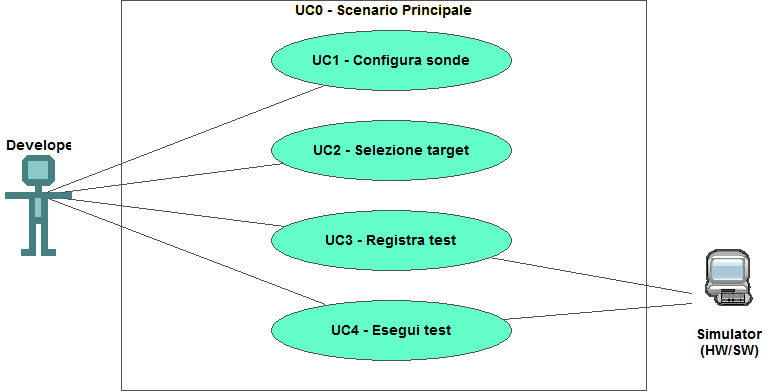
\includegraphics[width=0.9\columnwidth]{usecase/scenario-principale} 
    \caption{Use Case - UC0: Scenario principale}
\end{figure}

\begin{usecase}{0}{Scenario principale}
\usecaseactors{Sviluppatore applicativi}
\usecasepre{Lo sviluppatore è entrato nel plug-in di simulazione all'interno dell'IDE}
\usecasedesc{La finestra di simulazione mette a disposizione i comandi per configurare, registrare o eseguire un test}
\usecasepost{Il sistema è pronto per permettere una nuova interazione}
\label{uc:scenario-principale}
\end{usecase}

\section{Tracciamento dei requisiti}

Da un'attenta analisi dei requisiti e degli use case effettuata sul progetto è stata stilata la tabella che traccia i requisiti in rapporto agli use case.\\
Sono stati individuati diversi tipi di requisiti e si è quindi fatto utilizzo di un codice identificativo per distinguerli.\\
Il codice dei requisiti è così strutturato R(F/Q/V)(N/D/O) dove:
\begin{enumerate}
	\item[R =] requisito
    \item[F =] funzionale
    \item[Q =] qualitativo
    \item[V =] di vincolo
    \item[N =] obbligatorio (necessario)
    \item[D =] desiderabile
    \item[Z =] opzionale
\end{enumerate}
Nelle tabelle \ref{tab:requisiti-funzionali}, \ref{tab:requisiti-qualitativi} e \ref{tab:requisiti-vincolo} sono riassunti i requisiti e il loro tracciamento con gli use case delineati in fase di analisi.

\newpage

\begin{table}%
\caption{Tabella del tracciamento dei requisti funzionali}
\label{tab:requisiti-funzionali}
\begin{tabularx}{\textwidth}{lXl}
\hline\hline
\textbf{Requisito} & \textbf{Descrizione} & \textbf{Use Case}\\
\hline
RFN-1     & L'interfaccia permette di configurare il tipo di sonde del test & UC1 \\
\hline
\end{tabularx}
\end{table}%

\begin{table}%
\caption{Tabella del tracciamento dei requisiti qualitativi}
\label{tab:requisiti-qualitativi}
\begin{tabularx}{\textwidth}{lXl}
\hline\hline
\textbf{Requisito} & \textbf{Descrizione} & \textbf{Use Case}\\
\hline
RQD-1    & Le prestazioni del simulatore hardware deve garantire la giusta esecuzione dei test e non la generazione di falsi negativi & - \\
\hline
\end{tabularx}
\end{table}%

\begin{table}%
\caption{Tabella del tracciamento dei requisiti di vincolo}
\label{tab:requisiti-vincolo}
\begin{tabularx}{\textwidth}{lXl}
\hline\hline
\textbf{Requisito} & \textbf{Descrizione} & \textbf{Use Case}\\
\hline
RVO-1    & La libreria per l'esecuzione dei test automatici deve essere riutilizzabile & - \\
\hline
\end{tabularx}
\end{table}%

    % \chapter{Progettazione e codifica}
\label{cap:progettazione-codifica}

\intro{Breve introduzione al capitolo}\\

\section{Tecnologie e strumenti}
\label{sec:tecnologie-strumenti}

Di seguito viene data una panoramica delle tecnologie e strumenti utilizzati.

\subsection*{Tecnologia 1}
Descrizione Tecnologia 1.

\subsection*{Tecnologia 2}
Descrizione Tecnologia 2

\section{Ciclo di vita del software}
\label{sec:ciclo-vita-software}

\section{Progettazione}
\label{sec:progettazione}

\subsubsection{Namespace 1} %**************************
Descrizione namespace 1.

\begin{namespacedesc}
    \classdesc{Classe 1}{Descrizione classe 1}
    \classdesc{Classe 2}{Descrizione classe 2}
\end{namespacedesc}


\section{Design Pattern utilizzati}

\section{Codifica}

    % \chapter{Verifica e validazione}
\label{cap:verifica-validazione}

    \chapter{Conclusioni}
\label{cap:conclusioni}

\section{Raggiungimento degli obiettivi}
Il PoC sviluppato permette agli utenti la visualizzazione dei video e la possibilità di cambiare la qualità di visualizzazione, dà la possibilità agli espositori di caricare i video relativi ai propri prodotti e di gestirli e permette agli amministratori di gestire gli utenti, gli eventi e i video.\\
È stato sviluppato utilizzando le tecnologie richieste dall'azienda, in particolare React per il frontend, .NET Core per il backend e Azure per la gestione dei video e del database.\\
Inoltre sono stati sviluppati parzialmente gli unit test per il backend per verificare il corretto funzionamento delle funzionalità.\\
Successivamente è stata effettuata un analisi dei costi per il mantenimento dell'applicazione in base al numero di utenti utilizzatori dell'applicazione.\\
Infine è stata redatta la documentazione di resoconto finale, che descrive il lavoro svolto e i risultati ottenuti.\\
Concludendo, tutti gli obiettivi obbligatori sono stati raggiunti, tranne la realizzazione degli Unit Test completa del backend a causa di mancanza di tempo.\\
\section{Sviluppi futuri}
Il PoC sviluppato è una buona base per la realizzazione del prodotto finale, ma necessita di alcuni miglioramenti.\\
In particolare, l'aggiunta di un sistema di autenticazione per gli utenti, in modo da poter accedere all'applicazione solo se registrati, e di un sistema di autenticazione per gli espositori, in modo da poter caricare i video solo se autenticati.\\
Inoltre, sarebbe utile aggiungere un sistema di engagement per gli utenti, in modo da poter interagire con gli espositori e con gli altri utenti tramite commenti e valutazione dei prodotti.\\
Infine, è necessario aggiungere un sistema di controllo degli errori, in modo da poter gestire gli errori che possono verificarsi durante l'utilizzo dell'applicazione.\\

\section{Conoscenze acquisite}
Grazie a questa esperienza ho avuto l'opportunita di imparare nuove tecnologie come React, il framework .NET Core e il sistema di Azure, sicuramente molto utili per il mio futuro professionale. Inoltre, ho potuto approfondire le mie conoscenze in ambito di sviluppo web e di architetture software.\\
\section{Valutazione personale}
Sono molto soddisfatto del lavoro svolto, in particolare per la realizzazione del prototipo funzionante, che mi ha permesso di mettere in pratica le conoscenze acquisite durante il corso di studi e di imparare nuove tecnologie. Sicuramente il prodotto finale sarà molto utile per l'azienda presso la quale ho svolto tirocinio, in quanto ritengo sia una buona base dalla quale partire per la realizzazione del prodotto finale.\\ 
Questa esperienza ha confermato che il percorso di studi che ho scelto è quello giusto per me e mi ha approcciato verso il mondo del lavoro, che ho potuto conoscere meglio.\\

    % \appendix
    % \chapter{Appendice A}

\epigraph{Citazione}{Autore della citazione}


    % \backmatter
    % \printglossary[type=\acronymtype, title=Acronimi e abbreviazioni, toctitle=Acronimi e abbreviazioni]
    % \printglossary[type=main, title=Glossario, toctitle=Glossario]

    % \cleardoublepage
\chapter{Bibliografia}

\nocite{*}

% Print book bibliography
\printbibliography[heading=subbibliography,title={Riferimenti bibliografici},type=book]

% Print site bibliography
\printbibliography[heading=subbibliography,title={Siti web consultati},type=online]

\end{document}
